\chapter{blockchain aplicado a Federated Learning}\label{sec:blockfed}
Debido a las propiedades de la tecnología \textit{blockchain} han sido múltiples los trabajos para combinar \ac{FL} y esta tecnología~\cite{zhu-2023-blockfed} con el fin de resolver problemas causados mayormente por la centralización en \ac{FL}. La combinación de \textit{blockchain} y \ac{FL} es ampliamente usada  en múltiples campos~\cite{kim-2020-blockfl, weng-2021-deepchain} y ha mostrado un gran éxito que ha llevado a muchas propuestas. Aún así, como veremos, es un campo todavía muy reciente y por tanto sin ningún estándar establecido al que ceñirnos.

\section{Blockchain como solución a problemas del federated learning}

Una de las principales aplicaciones de la tecnología \textit{blockchain} en \ac{FL} es la propuesta de soluciones a algunos problemas derivados del aprendizaje distribuido en \ac{FL}. A continuación exponemos algunos de estos problemas vigentes en esquemas federados, muchos de ellos causados por la centralización de los esquemas clásicos de \ac{FL} y ofrecemos una breve vista sobre como el uso de tecnología \textit{blockchain} nos puede ayudar a solventar estos problemas o, al menos, mejorar las soluciones actuales.

\subsection{Falta de incentivos}
Cuando un cliente participa en una tarea de \ac{FL}, consume una cantidad de recursos, incluyendo computación, ancho de banda de la red y batería. Además son varios los riesgos de seguridad que suele llevar el esquema federado como hemos visto en secciones anteriores. Esto hace que en algunos casos los clientes no quieran formar parte de la tarea de \ac{FL} a no ser que obtengan un beneficio. 

Aunque los mecanismos de incentivo son un campo de investigación activo en \ac{FL}~\cite{wang-2018, xu-2015}, la mayoría de soluciones propuestas necesitan una entidad central en la que se pueda confiar para observar el comportamiento de los clientes y dar sus recompensas. Este problema proviene de la centralización del esquema de \ac{FL} y por tanto es un buen candidato a ser resuelto mediante el uso de \textit{blockchain}. El problema se puede resolver haciendo uso de los mecanismos de recompensa económicos que integran múltiples redes \textit{blockchain}. Por ejemplo, \citet{zhao-2021} propuso un sistema de reputación basado en \textit{blockchain} para \ac{FL} para dispositivos \ac{IoT} con el fin de entrenar modelos en los datos de los clientes.

\subsection{Heterogeneidad estadística}

La heterogeneidad estadística se refiere a las distintas distribuciones de datos de los clientes. Esto aumenta de manera drástica la complejidad del modelado del problema, análisis teórico y evaluación empírica de las soluciones. Por una parte, es difícil modelar los datos heterogéneos cuando se entrenan modelos federados en conjuntos no idénticamente distribuidos en los clientes. Por otro lado, no es fácil analizar la convergencia en procesos de entrenamiento en los que los datos son heterogéneos. En \textit{blockchain} se ha trabajado en algoritmos de optimización distribuidos logrando resolver las limitaciones de las soluciones existentes. Por ejemplo, el algoritmo de promedio con pesos según las distancias basado en \textit{blockchain} propuesto por~\citet{zhang-2021} ha demostrado tener una buena precisión a la hora de tratar el problema de heterogeneidad de datos en \ac{FL}. Además, se pueden desplegar redes \textit{blockchain}.

\subsection{Heterogeneidad de sistemas}
La heterogeneidad de sistemas se refiere a las diferencias sustanciales en capacidad de computación, ancho de banda de red, batería, capacidad de almacenamiento, etc., de los dispositivos en la red de \ac{FL}. Además, las restricciones del tamaño de la red de cada dispositivo o a nivel de sistema normalmente solo soportan un pequeño porcentaje de estos estando activos inmediatamente. Por lo tanto, una arquitectura de \ac{FL} debe de tolerar \textit{hardware} heterogéneo y ser lo suficientemente robusta como para descartar dispositivos en la red de comunicación. El uso de tecnología \textit{blockchain} también puede ayudar a abordar este problema. Un ejemplo es la propuesta de~\citet{zhang-2021} de un sistema de \ac{FL} basado en \textit{blockchain} para la detección de errores en dispositivos industriales \ac{IoT}, el cual puede lograr la integridad verificable de los datos de los clientes.

\subsection{Seguridad del modelo}
Como se mostró en la Sección~\ref{sec:ataquesfl} un esquema de \ac{FL} no es totalmente seguro y pueden participar clientes maliciosos con el fin de destruir los modelos finales. Además los modelos pueden ser filtrados por servidores no fiables llevando así también a problemas de privacidad. Las soluciones actuales no pueden eliminar la posibilidad de que un servidor central robe datos o modifique el modelo para dañarlo~\cite{zhu-2023-blockfed}. Los esquemas basados en \textit{blockchain} no requieren de un servidor central para la agregación del modelo lo que reduce riesgos en el sistema distribuido. Además, la verificación de identidad, trazabilidad, durabilidad, anonimidad y alta escabilidad de esta tecnología también permite garantizar la seguridad del modelo.

\subsection{Privacidad de los datos}
Aunque en \ac{FL} se compartan modelos y no datos, la comunicación de las actualizaciones del modelo entre clientes y servidor permite la extracción de información sensible a terceros o al servidor central. Además, algunos clientes maliciosos también pueden inferir información a partir de parámetros compartidos. Algunos métodos actuales pasan por el uso de \ac{DP} o métodos de  cifrado como vimos en la Sección~\ref{sec:fldp}, aunque tienen el problema de perjudicar el rendimiento del modelo. En métodos de \textit{blockchain} se ha propuesto con éxito~\cite{mcmahan-2018} la incorporación de \ac{DP} local a nivel de cliente. También la seguridad criptográfica de la \textit{blockchain} permite el cifrado del modelo global en la red dejando solo a los clientes con la clave para descifrar este, evitando así ataques externos.


\subsection{Coste de las comunicaciones}
Dado que el cómputo de entrenamiento está repartido entre dispositivos conectados a través de internet, las comunicaciones son un cuello de botella en una red federada. Una red federada puede contener gran cantidad de dispositivos diferentes, como millones de teléfonos móviles. Debido a los recursos limitados, como el bando de ancha de la red, energía o potencia, la comunicación en la red puede ser incluso más lenta que el cómputo local. Por lo tanto, es necesario desarrollar un método de comunicación eficaz. Se ha probado que usando un mecanismo de consenso adecuado y ajustando los parámetros básicos de la \textit{blockchain} se puede solventar este problema. Por ejemplo, en el trabajo propuesto por~\citet{kim-2020-blockfl} el sistema optimiza la latencia de fin a fin del modelo ajustando la tasa de generación de bloques de la red. Además, también propusieron un método para calcular la latencia mediante el ajuste de la dificultad en \ac{PoW}. \citet{majeed-2019} han empleado una \textit{blockchain} con permisos mejorando la eficiencia de transmisión significantemente.

\section{Mecanismos de consenso en blockchain aplicado a Federado}

Los mecanismos de consenso son un elemento clave de la arquitectura de la \textit{blockchain}. Aunque \ac{PoW} es todavía el principal método usado en este campo y el más estudiado en la literatura, tanto a nivel teórico como de propuestas de arquitecturas, no se considera práctico desplegar \ac{PoW} directamente en un sistema de \ac{FL} por motivos de eficiencia. Por lo tanto, esto ha llevado al diseño de varios métodos de consenso. Algunas propuestas usan \ac{PoS} como mecanismo de consenso~\cite{awan-2019, preuveneers-2018} debido a su bajo consumo energético aunque requieren el uso de algún mecanismo de incentivo económico, por lo que su uso es restringido. Una de las propuestas más interesantes es \ac{PoFL}~\cite{qu-2021-pofl}. 

El mecanismo de consenso \ac{PoFL}~\cite{qu-2021-pofl} fue desarrollado como solución eficiente a nivel energético para la integración de la tecnología blockchain con \ac{FL}. Inspirado por el concepto de los mecanismos de consenso \textit{Proof-of-Useful Work}~\cite{sabry-2023-pouw}, \ac{PoFL} mantiene la idea fundamental de \ac{PoW}: hacer que los participantes resuelvan problemas computacionalmente intensivos para lograr un consenso. Sin embargo, a diferencia de \ac{PoW}, que utiliza la potencia computacional para tareas sin ningún valor inherente (por ejemplo, encontrar un \textit{nonce} en la red de Bitcoin~\cite{duc-2023}), \ac{PoFL} decide usar estos recursos para entrenar un modelo federado.

\subsection{El mecanismo de consenso PoFL}
Es importante saber que \ac{PoFL} hace uso una arquitectura de \textit{pooled-mining}. En esta estructura, los participantes de la red son divididos entre diferentes \textit{pools}, cada una supervisada por un minero asignado. Estas \textit{pools} operan de manera independiente, entrenando sus respectivos modelos federados sin ninguna comunicación entre \textit{pools}. La \textit{pool} que entrene el modelo con mayor precisión en un conjunto de datos de prueba previamente determinado será considerada la ganadora en la ronda de consenso. Como consecuencia, el modelo ganador se integra en la blockchain y es retransmitido a través de toda la red a los clientes. El proceso dentro de cada \textit{pool} se ilustra en la figura \ref{fig:pooledmining}:
\begin{enumerate}
	\item El minero difunde el modelo inicial a los clientes.
	\item Los clientes entrenan su copia local del modelo usando sus datos privados. Este paso incluye el calcular las actualizaciones locales basadas en la diferencia entre el modelo recibido y el modelo entrenado.
	\item Los clientes mandan las actualizaciones locales al minero. El minero agrega estas actualizaciones para crear un nuevo modelo mejorado. El minero evalúa el rendimiento del modelo agregado contra una meta de rendimiento previamente establecida. Si se alcanza esta meta, se llega a consenso en esa ronda.
	\item Después de llegar al consenso, el minero añade el modelo mejorado a la blockchain y lo retransmite a todos los mineros, y por tanto a todos los clientes participando. Si no se llega a consenso (no se consigue la meta), el proceso se reinicia desde el paso 2, con los clientes entrenando hasta que se alcance la meta deseada.
\end{enumerate}

\begin{figure}[ht]
	\centering
	\usetikzlibrary{positioning}
\usetikzlibrary{calc}
\usetikzlibrary{babel}
\definecolor{pastelred}{HTML}{D37676}
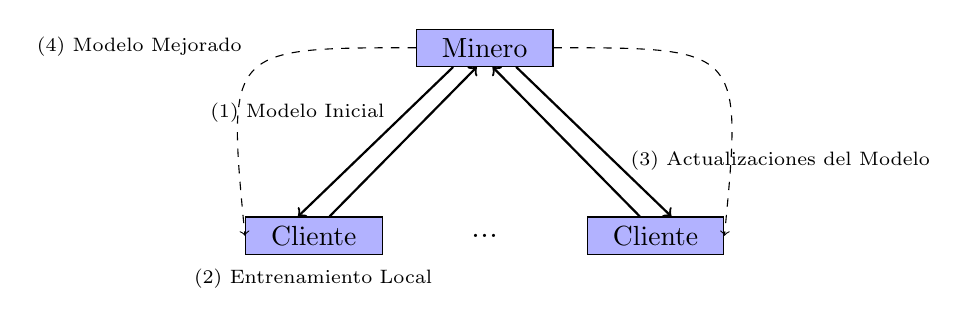
\begin{tikzpicture}[
scale=2,
clientnode/.style={rectangle, draw=black!100, text width=1.5cm,
align=center, anchor=center, fill=blue!30},
textnode/.style={}
]

%Nodes
\node[clientnode] (miner) {Minero};
\node[textnode] (dots) [below=2cm of miner] {\large ...};
\node[clientnode] (client1) [left=of dots] {Cliente};
\node[clientnode] (client2) [right=of dots] {Cliente};
\node[textnode] (label1) [below=0.05cm of client1] {\textsuperscript{(2) Entrenamiento Local}};
\node[textnode] (label2) [left=0.05cm of client2] {};

%Coordinates
\coordinate (miner1) at ($ (miner.south) - (0.2,0) $);
\coordinate (miner2) at ($ (miner.south) - (0.05,0) $);
\coordinate (miner3) at ($ (miner.south) + (0.05,0) $);
\coordinate (miner4) at ($ (miner.south) + (0.2,0) $);
\coordinate (client11) at ( $ (client1.north) - (0.1, 0) $ );
\coordinate (client12) at ( $ (client1.north) + (0.1, 0) $ );
\coordinate (client21) at ( $ (client2.north) - (0.1, 0) $ );
\coordinate (client22) at ( $ (client2.north) + (0.1, 0) $ );

%Lines
\draw[thick, ->] (miner1) -- (client11) node[midway, above left] {};
\draw[thick, ->] (miner4) -- (client22) node[midway, above right] {};
\draw[thick, ->] (client12) -- (miner2) node[midway, below right] {};
\draw[thick, ->] (client21) -- (miner3) node[midway, below left] {};

\draw[dashed, ->] (miner.west) .. controls +(left:1.2cm) .. (client1.west) node[midway, above left] {\textsuperscript{(4) Modelo Mejorado}};
\draw[dashed, ->] (miner.east) .. controls +(right:1.2cm) .. (client2.east) node[midway, above right] {};


\node[textnode, above=1cm of client11] {\textsuperscript{(1) Modelo Inicial}};
\node[textnode, above right=0.4cm and 3.7cm of client12] {\textsuperscript{(3) Actualizaciones del Modelo}};
    
\end{tikzpicture}
	\caption{Diagrama mostrando como funciona el procedimiento de \textit{pooled-mining}. Fuente: Elaboración propia.}
	\label{fig:pooledmining}
\end{figure}

Formalmente, podemos modelar una red de blockchain usando \ac{PoFL} como un conjunto de \textit{pools} $\{P_1, P_2, \ldots, P_n\}$, donde cada \textit{pool} $P_i$ contiene un minero $m_i$ y un conjunto de clientes $\{C_1^i, \ldots, C_{j_i}^i\}$. En cada ronda de aprendizaje $t$, cada \textit{pool} $P_i$ computa un modelo federado denotado por $L_i^t$ mediante un proceso de entrenamiento federado coordinado por e minero $m_i$. Entonces, cada minero $m_i$ calcula la precisión de su modelo $L_i^t$ en un conjunto de datos determinado $\mathcal{D}$, que denotaremos por $accuracy(L_i^t, \mathcal{D})$. El minero $m_i*$ ganará el consenso si
\begin{equation}
	accuracy(L_i^t, \mathcal{D}) \le accuracy(L_{i*}^t, \mathcal{D}) \quad \forall i \in \{ 1, \ldots, n\}.
\end{equation}

Después de llegar a consenso, el modelo $L_{i*}^t$ es difundido a todos los mineros $m_j$ con $j \ne i*$ los cuales comprobarán que la precisión calculada es correcta. Después de una verificación correcta, el minero $m_{i*}$ creará un nuevo bloque $b_t$ en que se establecerá $G^{t+1}=L_{i*}^t$ y la añadirá a la blockchain. Finalmente, todos los mineros descargarán la nueva versión de la blockchain y difundirán el nuevo modelo global $G^{t+1}$ a todos sus clientes, asegurándose así que todos los clientes tienen acceso al último modelo.


Aunque son varios los mecanismos propuestos la mayoría de estudios no están dedicados a escenarios de \ac{FL} por lo que su implementación puede no ser idónea para nuestro caso. Actualmente existe una alta demanda para desarrollar mecanismos de consenso eficientes a nivel energético para la redes \textit{blockchain} en \ac{FL}.

\section{Arquitecturas en blockchain aplicado a FL}

Debido a la amplia cantidad de arquitecturas propuestas, no han sido pocos los trabajos que han intentado categorizarlas. Una de las categorizaciones más interesantes es la de~\citet{zhu-2023-blockfed} que propone categorizar las arquitecturas según el conjunto de mineros y clientes de la red en tres tipos: desacoplado, acoplado y superpuesto. En lo que sigue $M$ hará referencia al conjunto de los mineros de la red y $C$ al conjunto de los clientes de la red.

\subsection{Modelo Desacoplado}
Se dice que nuestra red sigue un modelo desacoplado cuando dado un nodo, este solo trabaja en un esquema federado o en \textit{blockchain}, pero nunca en ambos. Formalmente se puede expresar como $C \cap M = \emptyset$. De este modo, los los clientes únicamente se encargarán de entrenar los modelos locales y de mandar las actualizaciones a los mineros. Estos últimos serán los encargados agregar los modelos, ejecutar el mecanismo de consenso, validar transacciones y escribir en la \textit{blockchain}. 

Este modelo tiene múltiples ventajas como la facilidad a la hora de su implementación o bajos requisitos energéticos para muchos nodos dado que no tienen que ejecutar el mecanismo de consenso todos. Sin embargo sí implica un mayor coste en comunicaciones, dificultad a la hora de implementar mecanismos de incentivo o seleccionar clientes adecuados.
\begin{figure}[h]
	\centering
	\includegraphics[width=0.8\textwidth]{figuras/decoupled.png}
	\caption{Esquema de una arquitectura según el modelo desacoplado. Fuente: \cite{zhu-2023-blockfed}.}
	\label{fig:decoupled}
\end{figure}

\subsection{Modelo Acoplado}
En el modelo acoplado, todos los nodos son responsables de participar en el esquema de \ac{FL} y de \textit{blockchain}. Formalmente se puede expresar como $C=M$. En este modelo, los nodos se pueden llamar nodos compuestos y realizan tanto el entrenamiento local como la agregación, generación de transacciones y verificación, sumando a esto la generación de bloques y su validación. 

Esto lleva a que los nodos tengan pocos costes de comunicaciones debido a la topología de la red. Además debido a la integración total de la \textit{blockchain} y el esquema federado, el modelo acoplado es también simple de configurar y de diseñar. Sin embargo, cada nodo realiza tareas intensivas a la hora de entrenar el modelo y de ejecutar el mecanismo de consenso. Otro problema es que cada nodo en el esquema tiene más responsabilidades que en otros esquemas, creando así más preocupaciones a nivel de privacidad de datos o seguridad del modelo.
\begin{figure}[h]
	\centering
	\includegraphics[width=0.8\textwidth]{figuras/coupled.png}
	\caption{Esquema de una arquitectura según el modelo acoplado. Fuente: \cite{zhu-2023-blockfed}.}
	\label{fig:coupled}
\end{figure}

\subsection{Modelo superpuesto}
En el modelo superpuesto encontramos tres tipos de nodos: nodos de \textit{blockchain}, nodos de \ac{FL} y nodos compuestos. Formalmente lo podemos expresar como $M \cap C \ne \emptyset, M\ne C$. Pese a las distintas funciones, un nodo puede cambiar su tipo a lo largo del tiempo. El modelo superpuesto equilibra el modelo acoplado y desacoplado y toma la ventajas de ambos. Sin embargo esto se ve reflejado en complejidad a la hora de configurar la red. 

La asignación de las funciones de los nodos se puede optimizar basado en los recursos disponibles, nivel de seguridad, etc. Sin embargo, a parte de las desventajas ya mencionadas, el modelo superpuesto tiene complicaciones a la hora de diseñar mecanismos de consenso e incentivo. Esto se debe a la dificultad intrínseca de la red.
\begin{figure}[h]
	\centering
	\includegraphics[width=0.8\textwidth]{figuras/overlapped.png}
	\caption{Esquema de una arquitectura según el modelo superpuesto. Fuente: \cite{zhu-2023-blockfed}.}
	\label{fig:overlapped}
\end{figure}

Como veremos más adelante, la mayoría de propuestas para combinar \ac{FL} y \textit{blockchain} consistirán en modelos acoplados o desacoplados que seguirán un estilo similar al de una red como \textit{Bitcoin}. Estas redes cuentan con lo que se conoce como mecanismo de \textit{Gossip}. Este mecanismo es un protocolo que permite a los mineros intercambiar información con el fin de que un minero $m_i$ pueda publicar en un bloque las transacciones recibidas o generadas por el minero $m_j$. Es por ello que la mayoría de arquitecturas se pueden ver como un esquema federado centralizado en el que en cada ronda $t$ el agregador central es un minero $m_{i_t}$. Este acercamiento nos permite beneficiarnos de todas las ventajas expuestas al principio del capítulo y con un diseño sencillo a nivel de red.